\documentclass{article}
\usepackage{graphicx,xy,amsmath,amssymb,amsthm,physics,mathtools,tcolorbox,hyperref}
\usepackage{xepersian}
\settextfont{XB Niloofar}
\title{	
	پیش گزارش پنجم درس آزمایشگاه اپتیک - دکتر مهدوی
	\\
	\small
	موضوع آزمايش: بررسی عدسی های ضخيم
	نوری
}
\author{
حسین محمدی 
\\
۹۶۱۰۱۰۳۵
}
\begin{document}
\maketitle
\section{کمیاتی که در روابط مربوط به عدسی ها با علامت مثبت و منفی جایگذاری می شوند و بررسی آن ها}
ابتدا پارامترهای موجود در یک مسئله را بایستی بشناسیم و سپس معین کنیم که هر کدام بسته به شرایط دارای چه علامتی هستند، ابتدا پارامترها را ببینید:
\begin{table}[h]
	\centering
	\caption{پارامترهای موجودر در یک مسئله ی شامل عدسی}
	\begin{tabular}{|c|c|c|c|c|}
		\hline
		کمیت & معنا \\
		\hline
		$s_0$ & فاصله جسم تا عدسی \\
		\hline
		$s_i$ & فاصله تصویر تا عدسی \\
		\hline
		$f$ & فاصله کانونی عدسی \\
		\hline
		$y_0$ & طول عمودی جسم \\
		\hline
		$y_i$ & طول عمودی تصویر \\
		\hline
		$x_0$ & فاصله شی تا یک کانون \\
		\hline
		$x_i$ & فاصله تصویر تا همان کانون \\
		\hline
		$M_T$ & بزرگنمایی عمودی عدسی \\
		\hline
	\end{tabular}
\end{table}
حالا بسته به این که تصویر یا شی مجازی یا حقیقی باشند ، می توان علامت های کمیت های بالا را معین کرد که در جدول زیر این علامت ها آمده اند:
\begin{table}[h]
	\centering
	\caption{ علامت پارامترهای موجودر در یک مسئله ی شامل عدسی}
	\begin{tabular}{|c|c|c|c|c|}
		\hline
		کمیت & + & - \\
	\hline
	$s_0$ & جسم حقیقی & جسم مجازی	\\ \hline
	$s_i$ & تصویر حقیقی & تصویر مجازی  \\ \hline
	$f$ & عدسی همگرا & عدسی واگرا\\ \hline
	$y_0$ & تصویر مستقیم & تصویر وارونه\\ \hline
	$y_i$ & تصویر مستقیم & تصویر وارونه\\ \hline
	$M_T$ & تصویر مستقیم& تصویر وارونه\\ \hline
	\end{tabular}
\end{table}

توجه کنید که منظور از «جسم مجازی» همان تصویر آینه یا عدسی های دیگر است.
\section{صفحه اصلی یا 
\lr{Principal Plane}
چیست و از آن چه استفاده ای می شود؟}
هرگاه دسته ای از پرتوهای موازی را به یک عدسی بتابانیم، یک دسته پرتو خروجی خواهیم داشت. حال پرتوهای خروجی و ورودی را امتداد دهیم تا یکدیگر را در نقاطی قطع کنند، مکان هندسی این نقاط تشکیل یک خم می دهد که برای عدسی های نازک این نقاط تشکیل یک صفحه در فضای سه بعدی می دهند، حال اگر مکان هندسی مذکور را برای عدسی های ضخیم رسم کنیم، خمی تشکیل می دهد که می توان آن را تقریبا یک صفحه در نظر گرفت.
به این صفحه 
\lr{First Principal Plane}
می گوییم. در شکل
\ref{Fig1}
شیوه به دست آوردن این محور را می بینید.
\begin{figure}[h]
	\centering
	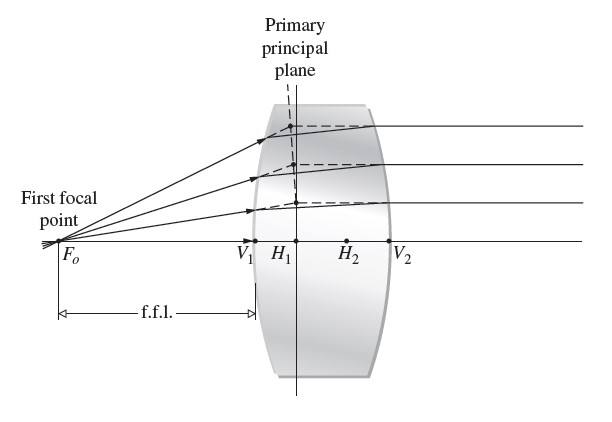
\includegraphics[scale=0.8]{1.jpg}
	\caption{بدست آوردن محور اصلی اول با کمک شکل}
	\label{Fig1}
\end{figure}

\noindent\\
حال پرتوهای ورودی را به گونه ای بتابانیم که پرتوهای خروجی موازی شوند؛ سپس مکان هندسی ذکر شده در بالا را به دست بیاوریم، به یک صفحه جدید می رسیم که به آن 
\lr{Second Principal Plane}
می گویند.
در شکل
\ref{Fig2}
شیوه به دست آوردن این محور را می بینید.
\begin{figure}[h]
	\centering
	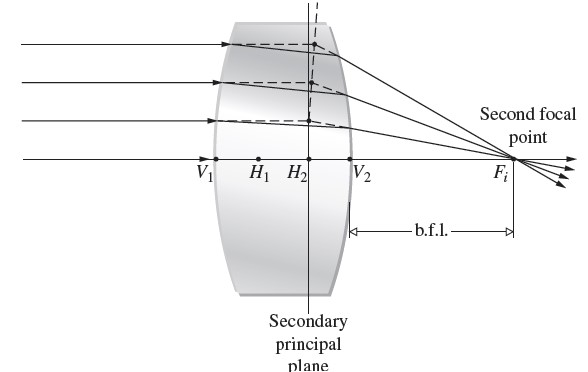
\includegraphics[scale=0.8]{3.jpg}
	\caption{بدست آوردن محور اصلی دوم با کمک شکل}
	\label{Fig2}
\end{figure}

\noindent\\
در حقیقت هدف از امتداد دادن پرتوها در بالا این است:«می توان به طور موثر در نظر گرفت که پرتوها در روی این صفحه ها شکسته یا بازتاب شده اند.» و می توان محاسبات و روابط مربوط به عدسی های ضخیم را به کمک بازتاب یا شکست از روی این صفحات انجام داد.
کاربرد بسیار جالب دیگری که در کتاب اپتیک هخت ذکر شده بود، دنبال کردن رد یک پرتو نور تابیده شده به یک عدسی ضخیم است. کافی است قوانین شکست نور را در این نقاط بنویسیم و رد یک پرتو نور را بررسی کنیم.
 
 \noindent\\
 در شکل 
 \ref{Fig3}
  محور اصلی را برای عدسی های ضخیم مختلف می بینیند:
 \begin{figure}[h]
 	\centering
 	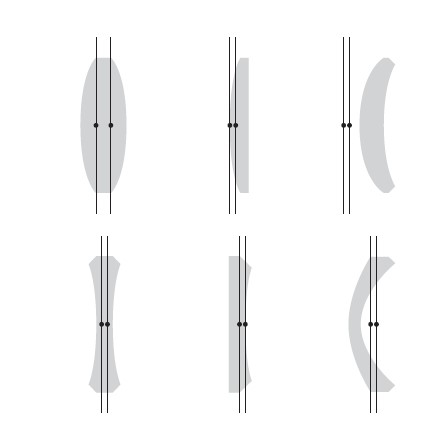
\includegraphics[scale=0.8]{2.jpg}
 	\caption{محورهای اصلی برای عدسی های ضخیم متفاوت}
 	\label{Fig3}
 \end{figure}





\end{document}